\documentclass[11pt,landscape,usenames,dvipsnames,letterpaper,leqno]{article}

%%%\nocolor

%\usepackage{equations,amssymb}
\usepackage{amsmath,amssymb,amsfonts}
\usepackage{graphicx,graphics}
\usepackage[pdftex]{color}
\usepackage{multirow} 
\usepackage{verbatim} 
\usepackage{ragged2e}

\usepackage{tikz}
\usetikzlibrary{matrix,arrows}
\usetikzlibrary{decorations.pathreplacing}
\usetikzlibrary{shapes.misc, positioning}

%\Large
\def\largesize{\normalsize}%\small}
\def\medsize{\footnotesize}
\def\smallsize{\scriptsize}
%\tiny

\definecolor{myblue}{rgb}{0,0,1}
\definecolor{myolivegreen}{cmyk}{.6,0,1,.25}
\definecolor{mymaroon}{cmyk}{0,1,1,.2}
\def\Maroon{\textcolor{mymaroon}}
\def\BurntOrange{\textcolor{BurntOrange}}
\def\Red{\textcolor{Red}}
\def\Blue{\textcolor{myblue}}
\def\Black{\textcolor{Black}}
\def\Brown{\textcolor{Brown}}
\def\PineGreen{\textcolor{PineGreen}}
\def\OliveGreen{\textcolor{myolivegreen}}
\def\Green{\textcolor{Green}}

\pagestyle{empty}
\raggedright
\hyphenpenalty=10000

\setlength{\textwidth}{10.2in}
\setlength{\textheight}{7.7in}

\setlength{\oddsidemargin}{-0.6in}
\setlength{\evensidemargin}{-0.6in}
\setlength{\topmargin}{-0.75in}
\setlength{\headsep}{0in}
\setlength{\headheight}{0in}

%------------------------------------------------------------------------------

\def\ds{\displaystyle}
\def\0{\phantom{0}}
\def\d{\partial}
\def\<{\langle}
\def\>{\rangle}
\def\qed{\qquad\Blue{\mbox{$\Box$}}}%QED}}

\def\grad{\nabla}
\def\div{\nabla\cdot}
\def\Div{\text{div}}
\def\curl{\nabla\times}
\def\Curl{\text{curl}}

\newcommand\red{\text{red}}

\def\argmin{\operatornamewithlimits{arg~min}}

\def\twoVec(#1,#2){\left(\begin{matrix}#1\\#2\end{matrix}\right)}

\fboxsep = 12pt
\def\myfbox#1{\Blue{\fbox{\Black{$\ds#1$}}}}
\def\myfboxMaroon#1{\Maroon{\fbox{\Black{$\ds#1$}}}}

\def\Line(#1,#2)(#3,#4){\qbezier(#1,#2)(#1,#2)(#3,#4)}

\def\picWidth#1#2%
{\includegraphics[clip=true,keepaspectratio=true,width=#1]{#2}}
\def\picHeight#1#2%
{\includegraphics[clip=true,keepaspectratio=true,height=#1]{#2}}
\def\picWidthHeight#1#2#3%
{\includegraphics[clip=true,width=#1,height=#2]{#3}}

%- - - - - - - - - - - - - - - - - - - - - - - - - - - - - - - - - - - - - - - - - - - - - -

\def\Re{\mathbb R}
\def\Bu{\mathbb B}
\def\Ed{\mathbb E}
\def\Po{\mathbb P}
\def\Su{\mathbb S}

\def\F{{\mathbf F}}
\def\u{{\mathbf u}}
\let\vv=\v
\def\v{{\mathbf v}}
\def\V{{\mathbf V}}
\def\x{{\mathbf x}}
\def\bpsi{{\boldsymbol\psi}}

%\def\cE{{\cal E}}
\def\cF{{\cal F}}
\def\cO{{\cal O}}
\def\cP{{\cal P}}
\def\cT{{\cal T}}

\def\RT{\text{RT}}
\def\AC{\text{AC}}
\def\BDM{\text{BDM}}
\def\myStrut{\vphantom{\int^H}}

%------------------------------------------------------------------------------
\newcommand\heading[1]{\medskip{\largesize\bf\Blue{#1}\par}}
\newcommand\head[1]{\medskip{\largesize\bf\Blue{#1}}}
\newcommand\subheading[1]{\smallskip{\it\Maroon{#1}}}
\newcommand\subhead[1]{\smallskip{\it\Maroon{#1}}}

\newcommand\eq[1]{\par\smallskip\centerline{$\ds#1$}\smallskip}

\let\itemOld=\item
\def\item{\parskip=0pt\itemsep=0pt\itemOld}

\newcounter{listNumber}
\newenvironment{nlist}
{\setcounter{listNumber}{0}
\list{\stepcounter{listNumber}\Blue{\thelistNumber.}}
{\leftmargin=16pt\topsep=0pt\parskip=0pt}}
{\endlist}

\newenvironment{blist}
{\list{\PineGreen{$\bullet$}}{\leftmargin=12pt\topsep=0pt\parskip=0pt}}
{\endlist}

\newenvironment{dlist}
{\list{}{\leftmargin=36pt\topsep=0pt\parskip=0pt}}
{\endlist}

%=====================================================================

\begin{document}
\parindent=0pt\medsize

\centerline{\vbox to0pt{\parbox{\textwidth}{\setlength\unitlength{1in}
\begin{picture}(10.2,7.7)(0,0)
\linethickness{2pt}
\put(-.1,-.1){\BurntOrange{\framebox(10.4,7.9){}}}
\end{picture}}\vss}}

\parbox{\textwidth}{
\parbox[t]{10in}{\centerline{\vbox{\halign{\hfil#\hfil\cr
{\Large\bf A Modified Bernardi-Raugel Element using}\cr
{\Large\bf  Direct Serendipity Space}\cr
\noalign{\smallskip}
\OliveGreen{{\em Todd Arbogast$^*$, and Chenyu Tian*$$}}\cr
\noalign{\smallskip}
\Brown{$^*$Oden Institute,
University of Texas at Austin}\cr}}}}\hfill}

\vspace*{-4pt}

% ====================================================================
\setlength{\abovedisplayskip}{3.5pt}
\setlength{\belowdisplayskip}{3.5pt}
\setlength{\abovedisplayshortskip}{3.5pt}
\setlength{\belowdisplayshortskip}{3.5pt}

\hbox to\textwidth\bgroup}{%
\parbox[t]{0.31\textwidth}{\raggedright
\head{Quadrilateral Mesh}

		  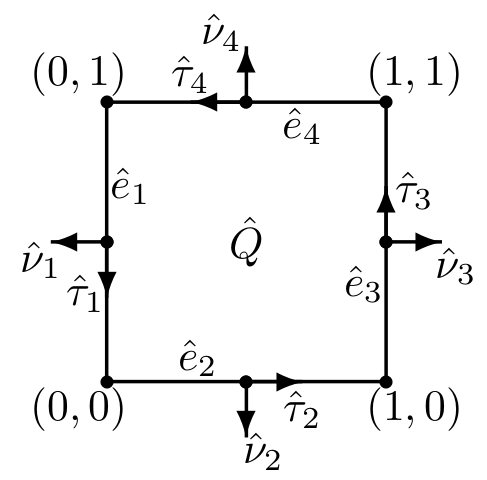
\includegraphics[width=3.5cm,height=3cm]{rec.png} 
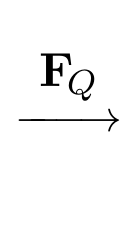
\includegraphics[width=0.8cm,height=2cm]{arrow.png}
		  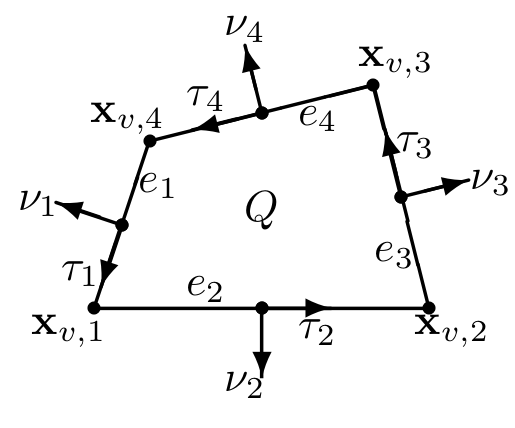
\includegraphics[width=3.5cm,height=3cm]{quad.png} 

\centerline{\vbox to0pt{\parbox{\textwidth}{\setlength\unitlength{1in}
\begin{picture}(0.2,0.7)(0,0)
\linethickness{1pt}
\setlength\fboxsep{0pt}
\put(-.05,.2){\colorbox{BurntOrange!10}{\BurntOrange{\framebox(3.15,0.57){}}}}
\end{picture}}\vss}}

\vspace{-.15in}
\head{\Black{Question}}\\
\vspace{.05in}
{Can we use Bernardi-Raugel element on quadrilateral mesh directly without mapping?}

\vspace{.2cm}
\head{First order Direct Serendipity Space}
\subhead{Auxiliary functions}\\
\vspace{0.1cm}
We index the edges $e_i$ in the counterclockwise direction, and define the outer
unit normal as $\nu_i$, tangents as $\tau_i$ and vertices as
$\mathbf{x}_{v,1}$, then define special linear function
$\lambda_i$ for $i = 1,2,3,4$.
\begin{equation*}
       \lambda_i(\x) = -(\x - \x_{vi})\cdot\nu_i,\quad i=1,2,3,4,
\end{equation*}
Then define
\begin{equation*}
        R_{13}(\x) = \frac{\lambda_1 - \lambda_3}{\lambda_1 + \lambda_3},\quad
        R_{24}(\x) = \frac{\lambda_2 - \lambda_4}{\lambda_2 + \lambda_4},
\end{equation*}
and
\begin{equation*}
		  \begin{aligned}
					 R_1(\x) &= \tfrac{1}{2}(1-R_{13}),\quad
        R_3(\x) = \tfrac{1}{2}(1+R_{13}),\\
					 R_2(\x) &= \tfrac{1}{2}(1-R_{24}),\quad
        R_4(\x) = \tfrac{1}{2}(1+R_{24}).
		  \end{aligned}
\end{equation*}
Function $R_i$ is 1 on corresponding edge $e_i$, 0 on the 
opposite edge, and arbitrary on two neighbours.
\begin{equation*}
    \mathbb{S}_1(Q) = \text{span}\big\{
        \lambda_2\lambda_4 R_{13},\ \lambda_1\lambda_3 R_{24}\big\},
\end{equation*}

\subhead{Resulted $\mathbb{DS}_1(Q)$ space}
\begin{equation*}
\mathbb{DS}_1(Q) = \mathbb{P}_1\oplus\mathbb{S}_1(Q),
\end{equation*}
Defined on the given quadrilateral $Q$.

\head{Modified Bernardi-Raugel finite element}
The modified Bernardi-Raugel finite element is
therefore defined as following:
\begin{equation*}
		  \begin{aligned}
					 \mathbb{V}_{S,h}(Q)&= \mathbb{DS}_1^2(Q)\oplus \text{span}\{\mathbf{b}_1, \mathbf{b}_2,\mathbf{b}_3, \mathbf{b}_4\}\\
					 \mathbb{W}_{D,h}(Q) &= \mathbb{W}_1^0(Q) = \mathbb{P}_0,
		  \end{aligned}
\end{equation*}

% ===================================================================

\vspace*{-8pt}}\hspace{.65cm}\parbox[t]{0.32\textwidth}{\raggedright

\subhead{Edge basis}\\
Four supplemental functions are defined modulo 4 by
\begin{equation*}
     \mathbf{b}_i(\x) = \frac{\varphi_{i}(\x)}{\varphi_{i}(\x_{i})} \nu_{i},\quad
     \x_i = \tfrac12(\x_{v,i-1}+\x_{v,i}),\quad
     \varphi_{i} = \lambda_{i+1}\lambda_{i+3}R_i,
\end{equation*}
We remark that the scalar function $\phi_i$ lie in second order
serendipity space $\mathbb{DS}_2(Q)$.

\subhead{Nodal basis}\\
Set auxiliary rational function first
\begin{equation*}
		  \begin{aligned}
					 r(\x) = &\frac{\lambda_3(\x)\lambda_4(\x)}{\lambda_3(\x_{v,1})\lambda_4(\x_{v,1})}-\frac{\lambda_1(\x)\lambda_4(\x)}{\lambda_1(\x_{v,2})\lambda_4(\x_{v,2})}+\\
					 &\frac{\lambda_1(\x)\lambda_2(\x)}{\lambda_1(\x_{v,3})\lambda_2(\x_{v,3})}-\frac{\lambda_2(\x)\lambda_3(\x)}{\lambda_2(\x_{v,4})\lambda_3(\x_{v,4})}
		  \end{aligned}
\end{equation*}
and then define
\begin{equation*}
    R(\x) = r(\x) - \sum_{i=1}^4r(\x_{e,i})\frac{\varphi_{i}(\x)}{\varphi_{i}(\x_{i})}.
\end{equation*}
Let $\nu_{d,i}$ be a unit normal to the first diagonal joining $\mathbf{x}_{v,i}$
with $\mathbf{x}_{v,i+2}$, and define new linear functions as
\begin{equation*}
    \lambda_{d,1} = -(\x - \x_{v,1})\cdot\nu_{d,1} \quad \text{and} \quad \lambda_{d,2} = -(\x-\x_{v,2})\cdot\nu_{d,2}.
\end{equation*}
Then the four nodal basis functions are defined as following
\begin{align*}
    \psi_{v,1}(\x) &= \frac{\lambda_{d,2}(\x) - \frac{1}{2}       \lambda_{d,2}(\x_{v,3})(1+R(\x))}{\lambda_{d,2}(\x_{v,1})-\lambda_{d,2}(\x_{v,3})},\\
    \psi_{v,2}(\x) &= \frac{\lambda_{d,1}(\x) - \frac{1}{2}       \lambda_{d,1}(\x_{v,4})(1+R(\x))}{\lambda_{d,1}(\x_{v,2})-\lambda_{d,1}(\x_{v,4})},\\
    \psi_{v,3}(\x) &= \frac{\lambda_{d,2}(\x) - \frac{1}{2}       \lambda_{d,2}(\x_{v,1})(1+R(\x))}{\lambda_{d,2}(\x_{v,3})-\lambda_{d,2}(\x_{v,1})},\\
    \psi_{v,4}(\x) &= \frac{\lambda_{d,1}(\x) - \frac{1}{2}       \lambda_{d,1}(\x_{v,2})(1+R(\x))}{\lambda_{d,1}(\x_{v,4})-\lambda_{d,1}(\x_{v,2})}.
\end{align*}

\head{An alternative definition of $R(\mathbf{x})$}\\
Redefine as modulo 4
\begin{equation*}
		  R_{i,i+1} = \frac{\lambda_{i-2}\lambda_{i-1}}{(\lambda_{i-2} + 
		  \alpha\lambda_{i})(\lambda_{i-1}+\beta\lambda_{i+1})}
\end{equation*}
where
\begin{equation*}
		  \alpha = -\frac{\tau \cdot \nu_{i}}{\tau \cdot \nu_{i+1}}, \quad 
		  \beta  = -\frac{(\mathbf{x}_{v,i} - \mathbf{x}_{v,i+1})\cdot \nu_{i-2}}{(\mathbf{x}_{v,i} - \mathbf{x}_{v,i+1})\cdot \nu_{i-1}}
\end{equation*}
Normalized as
\begin{equation*}
		  \tilde{R}_{i,i+1} = \frac{R_{i,i+1}}{\sum_{k=1}^{4}R_{k,k+1}}
\end{equation*}
% ======================================================================

\vspace*{-8pt}}\hspace{.5cm}\parbox[t]{0.32\textwidth}{\raggedright

Then the alternative $R(\mathbf{x})$ is defined
\begin{equation*}
		  R = \tilde{R}_{1,2} + \tilde{R}_{3,4} - \tilde{R}_{1,3} - \tilde{R}_{2,4}
\end{equation*}

\head{Preliminary numerical results}\\
Stokes equation with exact following solution
\begin{alignat*}2
&u = \cos(x)\sin(y), \quad && v= -\sin(x)\cos(y) \\
&\frac{\partial p}{\partial x} = \cos(x)\sin(y), \quad && \frac{\partial p}{\partial y}= \sin(x)\cos(y)
		 \end{alignat*}
\subhead{Rectangular Mesh}
\begin{center}
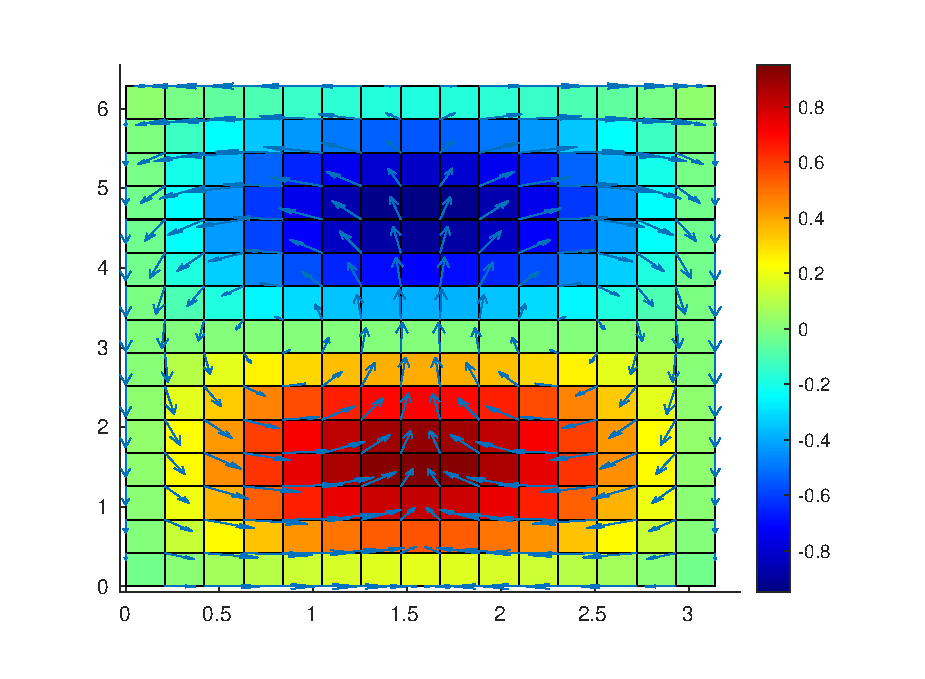
\includegraphics[width=6cm,height=3cm]{ex2.eps}
\end{center}
\begin{tabular}{c | c c c}
     Grid size & $16\times 16$ & $32\times32$ & $64 \times 64$ \\
     \hline
     $L^2(\text{res}_u)$ & $1.052\times10^{-1}$ & $2.513\times10^{-2}$ &$6.130\times10^{-3}$ \\
     $L^2(\text{res}_p)$ & $4.463\times10^{-1}$ & $2.093\times10^{-1}$ & $1.019\times10^{-1}$ \\
     $L^2(\text{res}_{du})$ & $5.845\times10^{-1}$ & $1.374\times10^{-1}$ & $3.330\times10^{-2}$ \\\end{tabular}   

\subhead{Quadrilateral Mesh}
\begin{center}
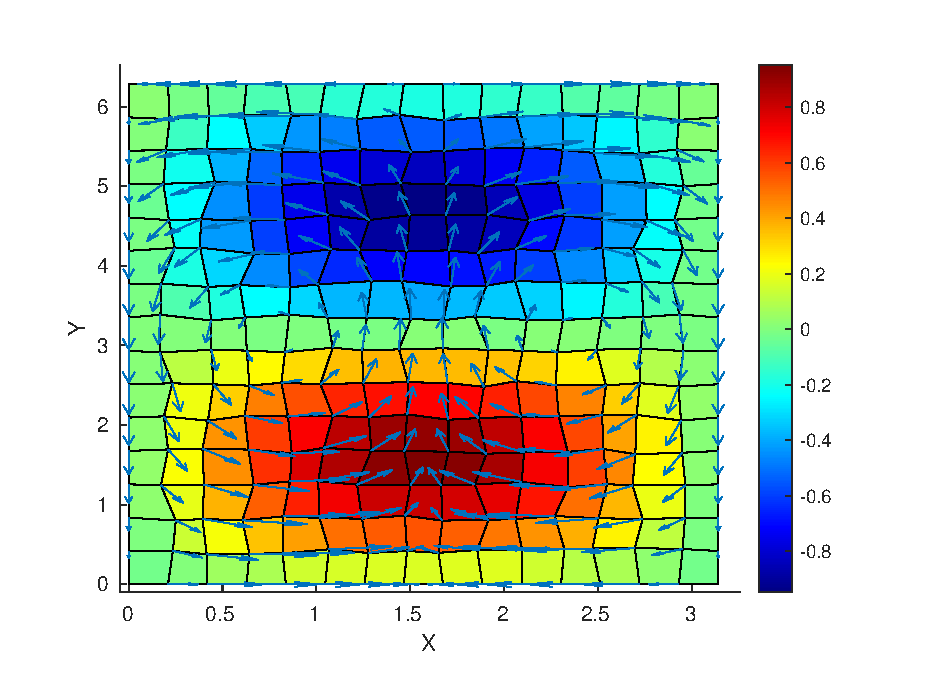
\includegraphics[width=6cm,height=3cm]{ex1.eps}
\end{center}

\begin{tabular}{c | c c c}
     Grid size & $16\times 16$ & $32\times32$ & $64 \times 64$ \\
     \hline
     $L^2(\text{res}_u)$ & $1.074\times10^{-2}$ & $2.567\times10^{-2}$ & $6.266\times10^{-3}$ \\
     $L^2(\text{res}_p)$ & $4.670\times10^{-1}$ & $2.207\times10^{-1}$ & $1.078\times10^{-1}$ \\
     $L^2(\text{res}_{du})$ & $5.981\times10^{-1}$ & $1.525\times10^{-1}$ & $4.580\times10^{-2}$ \\
\end{tabular}

\head{Summary}\\
\begin{nlist}
\item Achieves second order convergence on velocity, first order convergence on derivatives.
\item Same convergence rate achieved on both rectangular and quadrilateral mesh.
\end{nlist}


}

}
\end{document}
